% TODO: Devemos explicar como o fiscalizador eletrônico funciona? (https://industriahoje.com.br/como-funcionam-os-radares-de-velocidade)

% TODO: Mostrar falha nos dados que podem indicar coisas ruins, mas só falar como que vamos lidar no pré-processamento

% TODO: Adicionar gráficos de análise de dados como estacionaridade, sazonalidade e outros

% TODO: Usar a análise de dados do Fábio como inspiração

% TODO: Falar que não tem inconsitências muito grandes (perda de dados)

% TODO: Falar a quantidade de registros total e de que dia a que dia vão os dados

Neste capítulo, é apresentada uma análise do \textit{dataset} utilizado para estimar o nível de congestionamento da via urbana.




Este capítulo tem como objetivo realizar uma análise dos tipos de dados que estamos utilizando. Mostrar os desafio e problemas que tivemos que lidar ao tratá-los.

\section{Características do Tráfego}

É importante salientar que o tráfego é afetado por diversos fatores: temporais, espaciais e aleatórios. Os fatores temporais são, por exemplo, o horário do expediente dos trabalhadores que possuem veículos. Os fatores espaciais são, por exemplo, como a malha rodoviário se distribui em uma localização, ou a quantidade de empresas em uma área. Já fatores aleatórios são, por exemplo, acidentes que possam vir a ocorrer e a meteorologia do dia. Sendo assim, modelos de previsões podem ter desempenhos diferentes dependendo de onde e quando os dados forem coletados. Isso sem levar em conta a impossibilidade de se prever os fatores aleatórios.

Dessa forma, é comum na literatura optar-se por usar apenas dados com fatores espaciais e temporais. Assim fazendo uma suposição de que exista uma tendência no fluxo que pode ser previsto e que, embora as variáveis aleatórias possam afetar o fluxo, elas não afetam o bastante para mudar a tendência no longo prazo. Seguindo a literatura, esse artigo utilizará variáveis temporais e espaciais.


\section{Aquisição}

Os dados\footnote{http://bit.ly/processed-data-2l5MaAG} provêm de dois cruzamentos na avenida Hélio Prates que cruza Taguatinga e Ceilândia, duas cidades satélites do Distrito Federal (DF). Estes dados foram coletados e fornecidos pelo Departamento de Trânsito (\acrfull{DETRAN}\footnote{http://www.detran.df.gov.br/}) do \acrfull{DF}. Sendo a coleta feita por fiscalizadores eletrônicos localizados nos cruzamentos.

% TODO: colocar todos os fiscalizadores eletronicos
% TODO: consertar o intervalo que recebemos
% TODO: consertar quantidade de sensores
Nesses dados estão inclusos registros de todos os veículos que passaram pelo local nos meses de maio a junho de 2016 em forma de uma série temporal. Os registros são de 4 sensores em 4 vias diferentes. Para cada registro se tem uma identificação do fiscalizador eletrônico, data, hora, faixa de via, velocidade, limite de velocidade da via e tamanho do veículo, assim como mostrado na tabela \ref{table:data}.

\begin{table}[h]
    \begin{tabular}{ccccccc}
    \toprule
    \multicolumn{1}{l}{\textbf{Id Equipamento}} & \multicolumn{1}{l}{\textbf{Data}} & \multicolumn{1}{l}{\textbf{Hora}} & \multicolumn{1}{l}{\textbf{Faixa}} & \multicolumn{1}{l}{\textbf{km/h}} & \multicolumn{1}{l}{\textbf{km/h Max}} & \multicolumn{1}{l}{\textbf{Tamanho}} \\ 
    \midrule
    RSI128 & 2016/05/01 & 00:00:09 & 1 & 20 & 60 & 0 \\
    RSI131 & 2016/05/01 & 00:00:09 & 2 & 45 & 60 & 1.1 \\
    RSI132 & 2016/05/01 & 00:00:09 & 1 & 40 & 60 & 0 \\
    RSI131 & 2016/05/01 & 00:00:10 & 1 & 35 & 60 & 0.5 \\ 
    \bottomrule
    \end{tabular}
    \label{table:data}
    \caption{Exemplo dos dados recebidos coletados pelo \acrshort{DETRAN}}
\end{table}

Os dados foram obtidos de equipamentos de fiscalização eletrônica, os quais estão instalados em vias semafóricas. Por este motivo, é possível identificar momentos curtos onde não há fluxo de carros. Além disso, alguns dos equipamentos foram desativados por alguns momentos para receberem manutenções, resultando em alguns períodos mais longos sem registro de tráfego.

\begin{figure}[t]
    \centering
    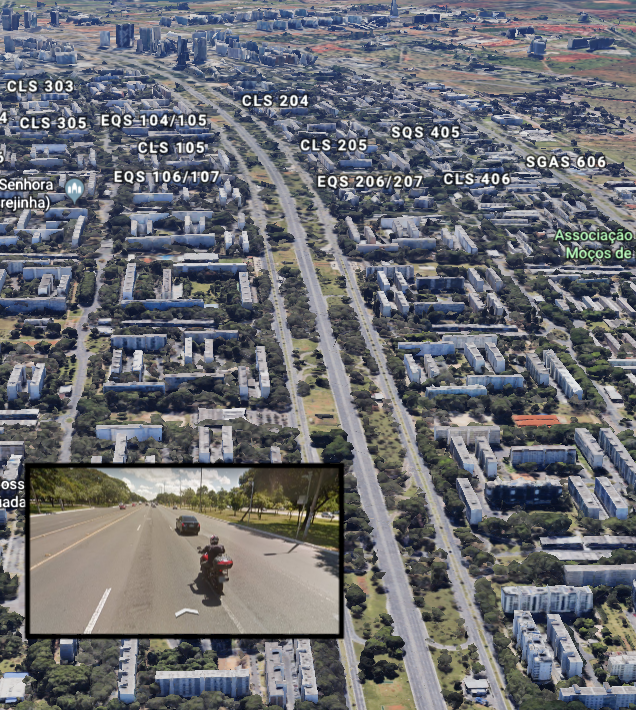
\includegraphics[scale=0.5]{street.png}
    \label{figure:eixo}
    \caption{Visão espacial do eixo monumental em Brasília}
\end{figure}


\section{Observações}


Também é válido dizer que, inicialmente, os dados possuíam mais uma coluna: tamanho do veículo. Esta, porém, foi descartada devido à suas inconsistências, como por exemplo, apresentar registros nos quais o tamanho do veículo era 0.

Por último, mas não menos importante, também deve-se notar que os fiscalizadores eletrônicos utilizados ficam próximos de semáforos, ou seja, existem momentos em que o fluxo diminui bastante, devido aos sinais vermelhos. 